\chapter{提案手法2}\label{method2}
\section{ヒューリスティックを用いるモデル}
より大規模な問題例を現実的な時間で解くために,ヒューリスティックを用いた数理モデルを提案する.

\subsection{ホールドの統合}
本研究では,ホールドの数が43の運搬船を考えている.
実オペレーションでは,それぞれのホールドを個別で考えるのではなく,複数のホールドをある程度まとめて考えて作業を行っている.
そのため,各階においてスロープのついているホールドを境目として,2つのホールドのまとまりとして考える.

複数のホールドを1つのまとまりとして考えると,43のホールドを,17のまとまりに統合することができる.このまとまりをセグメントと呼び,具体的な統合については
図\ref{fig1}に示す.

\begin{figure}[htbp]
 \centering
 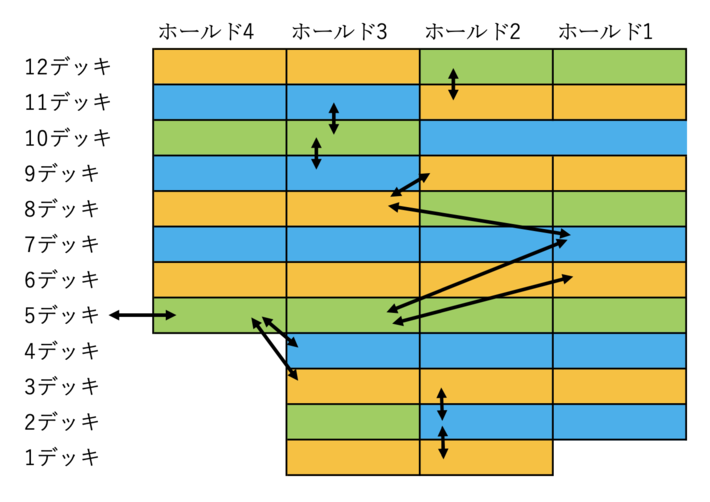
\includegraphics[width=0.9\linewidth]{segment.png}
 \caption{統合後のホールドを色付けしたもの}
 \label{fig1}
\end{figure}

\subsection{解の表現方法}
鵜川らによる研究の数理モデル\cite{ukawa}では,ホールドに注文を何台割り当てる,という連続的な解の表現方法を用いていた.
ヒューリスティックモデルでは,このような連続的な解表現方法を用いず,注文のセグメントへの割当のみを最適化し,詳細な車両の積載は決め打ちのルールを基に行っていく.
積載のルールは,ホールドの積載可能量,許容充填率などを満たすように設計を行っていく.

このように積載貨物を決めていくことで,注文を複数のホールドに渡って分割する場合であっても,隣接したホールドに車両を積むことができるため,プランナーの考える割当に近い解を出力することができる.

\section{提案手法}
\subsection{局所探索法}
局所探索法とは, ある解に少しの変更を加え得た近傍解が元の解よりも良い解である場合に, 変更後の解に移動するという操作を良い解が見つからなくなるまで繰り返す方法である.
変形を加える操作を近傍操作と呼び, 近傍内に改善解を持たない解を局所最適解と呼ぶ.

\subsection{初期解の生成}
\label{初期解}
各セグメントに対して,すべての注文をランダムに割り当てたものを用いる.

\subsection{近傍操作}
近傍操作には挿入近傍操作と交換近傍操作を用いる.

挿入近傍操作は,セグメントに割り当てられている注文の1つを,ランダムに異なるセグメントに挿入する操作である.
交換近傍操作は,異なるセグメントに割り当てられている注文を2つランダムに選び,それらを入れ替える操作である.

本研究では,はじめに挿入近傍操作を改善がなくなるまで繰り返し,その後交換近傍操作を改善がなくなるまで行う.
挿入近傍操作で1回でも改善があった場合は,再び挿入近傍操作からやり直す.

\subsection{評価関数}
評価関数では,数理モデル\cite{ukawa}の目的関数を用いる.
また,貨物の重量バランスに関する制約などに違反している場合には,制約違反度合いをペナルティ関数として表し, 目的関数に加えて探索を行う.

\subsection{近傍操作における計算時間の短縮}
\label{近傍操作の計算時間短縮}
本研究では,局所探索における近傍操作の1つとして挿入近傍操作を用いるが,操作に工夫を加えることで解の精度を変化させることなく計算時間を短縮させることができると考えられる.

挿入近傍操作では,1つの注文を異なるセグメントに挿入する.その際に,挿入可能な位置すべてを探索し評価関数の値が最も良くなる位置に挿入する.

しかし,あるセグメントに格納される注文の順番が変化しても評価関数の値が全く変化しない場合がある.そのような場合にはすべての挿入可能位置を探索する必要がないため,計算時間を短縮することができる.

以下に計算時間を短縮する提案手法の概要を示す.

\begin{algorithm}
 \caption{計算時間を短縮する手法}
 \label{algo1}
 \begin{algorithmic}[1]%1を0にすると行番号なし.
  \STATE あるセグメントから,注文を1つ選択する
  \STATE 挿入先のセグメントの,一番最後の位置に挿入する
  \STATE 複数のセグメントに分割された注文を$J_{\rm split}$とする.
  \FOR {$j \in J_{\rm split}$}
  \STATE $j$の前後に注文を挿入する
  \IF {評価関数の値が暫定解よりも良い}
  \STATE 暫定解を更新
  \ENDIF
  \ENDFOR
  \IF {暫定解が探索における最良解よりも良い}
  \STATE 最良解を更新
  \ENDIF
 \end{algorithmic}
\end{algorithm}
